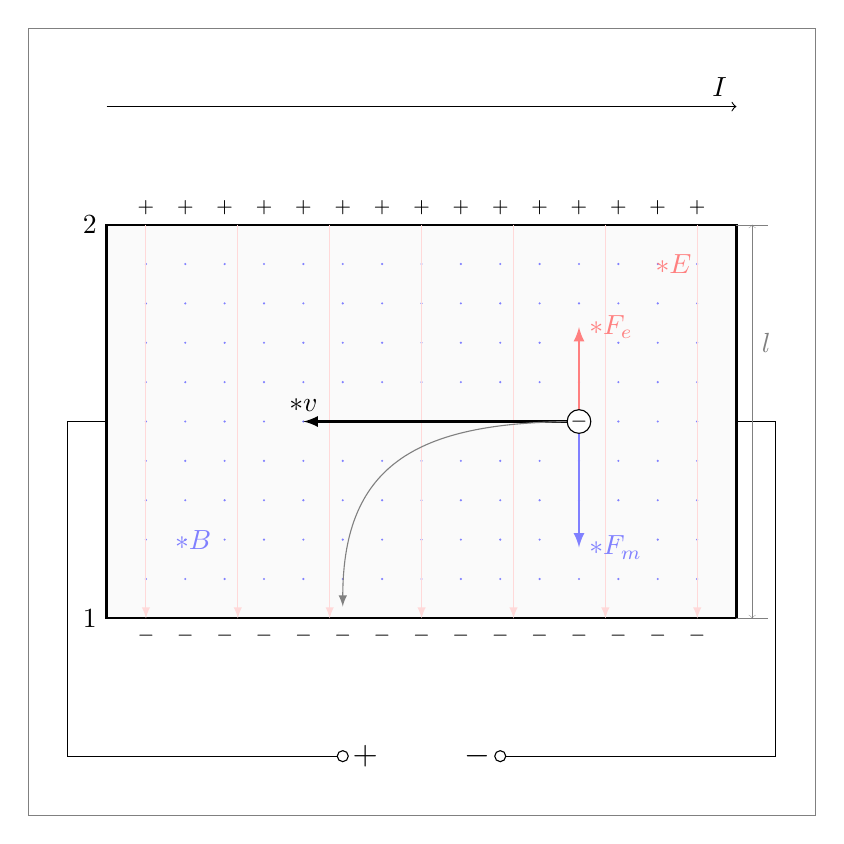
\begin{tikzpicture}[scale=1]
    \draw[gray,ultra thin] (-5,-5) rectangle (5,5);

    \draw[thick,fill=black!2!white] (-4,-2.5) rectangle (4,2.5);

    \foreach \x in {-3.5,-3,...,3.5}
    {
        \node[above] at (\x,+2.5) {\scriptsize $+$};
        \node[below] at (\x,-2.5) {\scriptsize $-$};
    }

    \foreach \x in {+3.50,+3.00,...,-3.50}
    {
        \foreach \y in {-2.0,-1.5,...,2.0}
        {
            \fill[blue!50!white] (\x,\y) circle (0.015);
        }
    }
    \foreach \y in {-3.50,-2.333,...,3.51}
    {
        \draw[red!15!white,-latex] (\y,2.5)--(\y,-2.5);
    }

    \node[blue!50!white] at (-2.9,-1.5) {$\vb*{B}$};
    \node[red!50!white]  at (+3.2,2) {$\vb*{E}$};

    \draw[-latex,thick](2,0)--(-1.5,0) node[above] {$\vb*{v}$};
    \draw[-latex,blue!50!white,thick](2,0)--(2,-1.6) node[right] {$\vb*{F}_m$};
    \draw[-latex,red!50!white,thick] (2,0)--(2,+1.2) node[right] {$\vb*{F}_e$};
    \draw[-latex,thin,gray](2,0).. controls (0,0) and (-1,-0.5) .. (-1,-2.35);
    \draw[fill=white] (2,0) circle (0.15) node {\scriptsize $-$};

    \draw (-4,0)--(-4.5,0)--(-4.5,-4.25)--(-1,-4.25);
    \draw[fill=white] (-1,-4.25) circle (0.07) node[right] {\large $+$};
    \draw (+4,0)--(+4.5,0)--(+4.5,-4.25)--(+1,-4.25);
    \draw[fill=white] (+1,-4.25) circle (0.07) node[left] {\large $-$};

    \draw[->](-4,4)--(4,4) node[above left] {$I$};
    \node[left] at (-4,-2.5) {$1$};
    \node[left] at (-4,+2.5) {$2$};

    \draw[gray,ultra thin] (4,2.5)--(4.4,2.5);
    \draw[gray,ultra thin] (4,-2.5)--(4.4,-2.5);
    \draw[gray,ultra thin,<->] (4.2,-2.5)--(4.2,+2.5);
    \node[gray,right] at (4.2,1) {$l$};
\end{tikzpicture}
